\chapter{Porting BaseX to the Android platform}
\label{sec:migration:porting-basex-to-android}
In this chapter it is shown how the BaseX database has been migrated to the Android platform.
To achieve this goal the source and target platforms are analyzed and all requirements are determined.
This includes the different software platforms and not the hardware specific aspects. 
In chapter~\ref{sec:migration:problems-during-the-migration} it is illustrated which parts of the BaseX version has been changed and how.
The last chapter describes the problems which are occurred during the migration.


\section{Analyzing the source and target platforms} 
\label{sec:migration:analysing-the-source-and-target-platform}
In this section the two different platforms are analyzed.
The main part of it is the software part, because both platforms are running on a huge amount of hardware devices.
The source platform is the Java Virtual Machine(JVM) and the target platform is the Dalvik Virtual Machine(Dalvik VM, or DVM) in the Android environment.
The JVM and the DVM are both virtual machines, but they vary in different ways.
One of the main difference is that the JVM is a stack based and the DVM is a register based virtual machine.
Also the DVM is optimized to be executed on mobile devices, which means that it is designed to use less memory and CPU usage than the JVM.
Lesser hardware usage implies also lesser battery usage, which is also a factor which should be considered in the field of mobile development.
Another difference which need to be considered is the host system, which is in the DVM case Android.
And for the JVM it could be Windows, Mac OS, or any Linux/Unix derivate. 
This need to be considered if external sources will be used, like writing or reading a file.


\subsection{Comparison of the two virtual machines}
\label{sec:migration:comparison-of-the-two-virtual-machines}
Like in the chapter before mentioned both source and target platforms are using Java as a programming language.
Compared to other general purpose programming languages, like C++, Java is not being compiled into machine code.
To execute Java code a virtual machine is required, which runs the compiled Java code.
However, like in Section~\ref{sec:migration:analysing-the-source-and-target-platform} mentioned both platforms have different virtual machines.
They differ in many kinds that the application developer not sees but need to consider.
\\
On of the most important difference is that the JVM is stack and the DVM is a register based virtual machine.
This difference helps the DVM to execute the same code in lesser operations than the JVM.
This means that the DVM need lesser CPU cycles than the JVM, which is an improvement that is necessary because of the lack of CPU resources in mobile devices and the aspect of the battery usage.
This can be demonstrated by looking at the instructions done by adding two integers.
The stack based virtual machine has to do four machine instructions, while the register based VM can do the operation in one instruction.
The reason for this is that the stack based VM needs to pop the two values first before it can add them and store them on the stack.
Figure~\ref{fig:stack-based-addition} illustrates the executed instructions of a addition with a stack based VM.
\begin{figure}[h]
\begin{center}
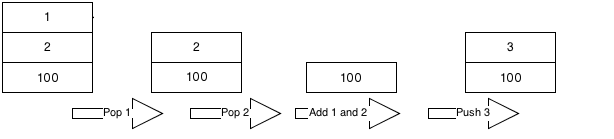
\includegraphics[scale=0.65]{images/stack-based-addition.png} 
\caption{The addition of two integers on a stack based virtual machine.}
\label{fig:stack-based-addition}
\end{center}
\end{figure}
Compared to this, the register based virtual machine just need one  machine instruction to complete the addition of two numbers.
The needed instruction is \textit{ADD R1, R2, R3}, which can be translated into add content of register 1 and register 2 and store it in register 3.
Figure~\ref{fig:register-based-addition} illustrates this by showing the add operation of the numbers one and two.
\begin{figure}[h]
\begin{center}
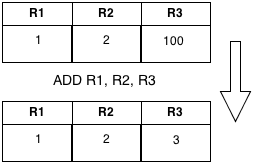
\includegraphics[scale=0.65]{images/register-based-addition.png} 
\caption{The addition of two integers on a register based virtual machine.}
\label{fig:register-based-addition}
\end{center}
\end{figure}
This minimal example shows how the register based virtual machine uses lesser machine instructions compared to the stack based.
The disadvantage in this is that register based machine has to store the addresses, the registers, of the operands.
Which is not necessary at a stack based machine, because of the stack pointer that always directs to the actual operand using the Last In First Out (LIFO) principal.
This leads to the result, that stack based code is smaller than the corresponding register based code.
Although the Dalvik VM is a register based virtual machine, the executed byte code is not bigger than the equivalent JVM code.~\cite{shi2008virtual}\\
This is the result of the different format of the executable virtual machine code, which is illustrated in Chapter~\ref{sec:comparison-of-the-two-bytecode-formats}.
\\
The performed instructions which are executed on Dalvik VM are called bytecode.
To execute this instructions the DVM has an interpreter which interprets all instructions and performs them.
This is an usual way how a virtual machine is implemented, but interpreters are slower than normal compiled machine code.
There is a technique which can improve a virtual machine in performance aspects by adding a Just In Time (JIT) compiler to it.
Generally it can be said, that a JIT compiler, used by a virtual machine, compiles heavy used code segments or very expensive calculations into machine code.
There are two types of JIT functioning:
\begin{itemize}
\item method-based
\item trace-based
\end{itemize}
The trace-based method works by looking at the most executed code fragments, especially loops, and compiles them into native machine code.
The method-based JIT mechanism is to compile whole methods, that are generally used and expensive in execution time.
Since the release of the Android version 2.2, codename Froyo, the Dalvik VM has received a JIT compiler additionally to the interpreter mechanism.
According to \cite{cheng2010jit} the implemented Dalivk JIT compiler can speed up the execution of intensive operations up to five times.
The Dalvik VM uses the above mentioned mechanism of a trace-based JIT compiler mixed with the usual DVM interpreter.
To realize this the DVM has received an additional thread, which is responsible for the JIT compilation.
This thread just compiles instructions from the trace queue, which gets generated by the main thread that counts the executions of the bytecode statements.\cite{oh2012evaluation}
Picture~\ref{fig:dvm-threads} illustrates the principle of the two threads in the DVM.
\begin{figure}[h]
\begin{center}
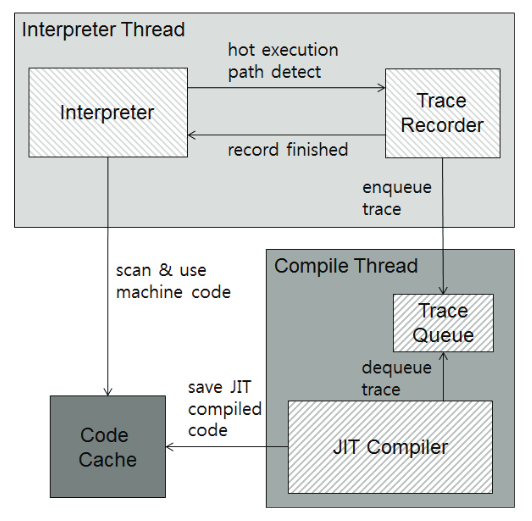
\includegraphics[scale=0.5]{images/dvm-threads.png} 
\caption{The principle of the two DVM threads. Source:\cite{oh2012evaluation}}
\label{fig:dvm-threads}
\end{center}
\end{figure}

The JVM has also a JIT compiler, but instead of a trace-based, like in the DVM, it uses method-based one.~\cite{kotzmann2008design}



\subsection{Comparison of the two byte code formats}
\label{sec:comparison-of-the-two-bytecode-formats}
Both virtual machines differ in their format of the executable files.
This is on one side the Java Archive File (JAR) for the JVM and the Android Application package file (APK) on the other side.
A JAR file is an archive which includes the compressed class files, this class files are being build out of the Java source code by using the javac compiler.~\cite{pugh1999compressing} 
An APK file is also an archive file, but it not only includes the executable program, it also includes the meta information and resource files.
The executable which includes an APK is called DEX file, which is short for Dalvik Executable.
A DEX file is created by using a tool which compiles Java class files into DEX files.
Picture~\ref{fig:create-apk} illustrates the flow of an APK creation, which differs to the creation of a JAR file by creating dex files out of the class files.\\
\begin{figure}[h]
\begin{center}
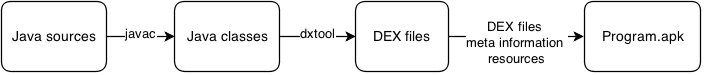
\includegraphics[scale=0.55]{images/create-apk.png} 
\caption{The creation flow of an APK file.}
\label{fig:create-apk}
\end{center}
\end{figure}

Having a closer look at the DEX files and comparing them to the JAR files shows that they differ in various ways.
The first thing that comes in mind is that a JAR file contains a class file for every class.
And a DEX file combines all specific information into one field.
For example it just has one constant pool, where all constant values of all classes are stored.
This includes integers, strings, method- and class references, for example.
Thinking about an interface which is used very often in a project can display what an advantage of one shared constant pool gives.
Looking at Image~\ref{fig:jar-dex} demonstrates that every class which uses this interface needs has its own reference in its own constant pool.
In general it can be said that DEX files are smaller than their equivalent JAR files.~\cite{bornstein2008dalvik}\\
\begin{figure}[h]
\begin{center}
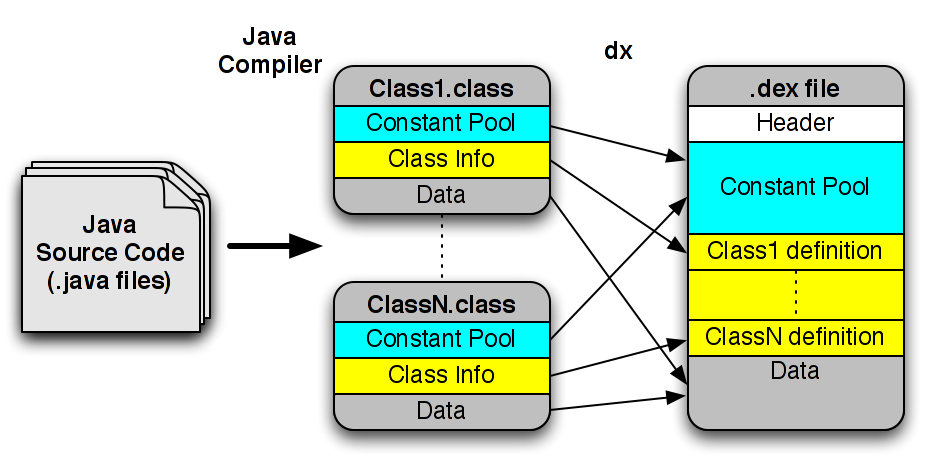
\includegraphics[scale=0.41]{images/jar-dex.png} 
\caption{The difference between a jar and a dex file. Source:~\cite{enck2011study}}
\label{fig:jar-dex}
\end{center}
\end{figure}

%\cite{ehringer2010dalvik}


\subsection{Requirements of the target platform}
\label{sec:migration:requirmenets-of.the-target-platform}
However, like the source platform the target platform uses also Java as programming language there are some differences which need to be considered.
To get an executable BaseX Android Version some adjustments need to be done.
It need to be considered that the Dalvik VM runs on mobile devices which are using Android as operating system.
Android is a Linux fork, but differs in some ways to the normal Linux operating system.
Android is optimized for mobile devices, which means that it does not require many hardware resources.
Also the process management differs in some ways. 
Android uses the Linux user management system to organize its applications and their privileges.
Every application is a own user and has its own sandbox, with every needed resources.
Although there are some ways it is usually not possible to access the sandbox of another application.
These interprocess communications (IPC) are provided by the Android operating system and are restricted in some ways.
They are usually used to provide information or notify other applications.
Like in Linux, where every user gets its own home directory, in Android every application gets its own directory in the /data/data/application directory.
In this directory the application stores all its data and this directory is only accessible by the application.
For this reason it is necessary that all files which were created and used by Basex are stored in this directory.
It would be also possible to store the data on an external storage, like a SD-Card, and limit the file rights.
By using this way, the problem is, that the IO operations on an external storage device are very expensive and slow.
Another constraint is the available Java libraries, depending on the API-Level Android does not offer so many like the standard Java version.
Some additional libraries can be added, if they only use the normal Java libraries.

\section{Changes of the source platform}
\label{sec:migration:changes-of-the-source-platform}
For the migration an Android project has been created, this provides all needed files.
To create an Android project the Android Software Development Kit(SDK) is necessary.
This can be downloaded on the official homepage of Android\footnote{\url{developer.android.com/sdk/index.html}}
The Android SDK, which is also called Android Developer Tools(ADT), provides many useful tools and also a plugin for the Eclipse IDE.
To create the BaseX library project the Eclipse create new project wizard has been used.
It is possible to mark the project as a library, this implies that the compiler creates a jar file out of the project.
The purpose of this is that the BaseX library can be used in every Android project by just including it.
All private data is stored in the /data/data/packagename directory.
So the method not just only creates an instance or returns the existing, it also checks if the private folder of the application is available and creates it if not.
If this folder has been created there is also a subfolder created which is called BaseXData.
This subfolder stores all databases created by the application and no other application can neither read nor write on this folder.
The next necessary change is to adjust the path on the Prop.java file.
This contains a static class that holds every property of the BaseX database, hence also the path to the database.
This has to be done before anything can read the filepath, so it is part of the constructor call.
BaseX provides methods that can be used to access, create, modify or delete the database.
For every of these operations a method inside the class has been created and can be called from outside.
Every method checks if a BaseX context is available, which should usualy be the case, and then executes the wanted operation.
Therefore the BaseX context is necessary and is used to make the specific operation on the database.
Every method in the class throws an IOException when something goes wrong, this exception comes from BaseX and need to be handled by the application which uses the library.
The reason why the directory name of the application has to be used at the constructor call is that it is not possible to get the name of the application inside the library.
There are methods provided by Android to receive the project package name, but this is the name of the package of the library.
And the library is not an application and therefore has no own data directory in the /data/data folder.
And it is not possible to create a own folder in this directory, because Android is doing it when the Application is being installed.
It would be also always the same folder, because 



%Android uses a different kind for generating UI objects than the standard Java version.
%This uses AWT and Swing, but these API aren't available on Android, so this can not be used on Android.
%Another difference between Android and the standard BaseX version is that Android has no user directory.
%Every application has its own directory which is located in /data/data/packagename.
%Therefore all files need to be stored there. 
%BaseX Android should be a library which means that every developer can use it.
%Therefore it is not known how the absolute path name is, because it is the package name of the executing activity.
%And this name differs from project to project.
%Therefore there is just one entry point for the library which is the class BaseXAndroid.
%The constructor of this class has a string argument, this parameter should be the absolute path to data directory of the application.
%To get this needed information the function getApplicationInfo().dataDir, which is inherited from the activity class, can be used in every activity of the application.




\section{Problems during the migration}
\label{sec:migration:problems-during-the-migration}
There occurred several problems during the migration.
The first problem which was discovered, was that some included libraries are not available on Android.
The following library couldn't be migrated because it is included in the JavaSE and is not available for Android.
\textit{crypto javax.xml.crypto}
BaseX identifies the operating system as Linux and then tries to save all BaseX related data into the home directory, which doesn't exist on Android.
This need to be, like in Section~\ref{sec:migration:requirmenets-of.the-target-platform} described the /data/data/application directory.
The problem hereby is that the goal of the migration is that the database is a library, but the directory name depends from the application name.
The only way to get the application way, except for hard coding, is to get the application context and extract the name there.
This bears another problem, though only applications have a context, libraries not. 
A possible way, could be to pass the context to the library, but then the library holds the context and just need to application name.
Holding a context massively slows down an Android application, so this is not the way how it was solved.
The alternative is to pass a string holding the application name to the library constructor and the library uses it to generate the needed directories.
This is also the way how it is done in the BaseX library.
To create a library object it is necessary to pass a string as an argument to the constructor.
Is this the first time an object of BaseX was created it tries to create the needed directory, /data/data/application-name/BaseXData.
In this directory all created databases and their depending files are stored.
\\
Another problem which occurred, was that BaseX uses a lot of the String function isEmpty(), which is not available at API-Level lower than 9.
The same applies for the copyOf() method in the java.util.Arrays package.
This was solved by not supporting API-level lower than 9 with BaseX library. 
The reason for this is that only 4\% of the used Android devices are using API-level lower than 9.
\\
After this adjustments it is possible to create a BaseX object on Android.
To get a library which supports all needed operations some more work was done.



